\section{离散无记忆信道}
\label{sec:dcc-dmc}

发送端送出一个符号，接收端收到另一个符号，两者之间的关系不确定但有规律。数学上，这种规律就是给定输入时输出的条件分布。先看三个二元输入的例子，它们在全章反复出现。

\paragraph{三个例子}
\term{二元对称信道}（binary symmetric channel，BSC）的输入、输出都是$\{0,1\}$，每个符号独立地以概率$p$被翻转，以概率$1-p$原样到达。\term{二元擦除信道}（binary erasure channel，BEC）的输出多一个符号$\mathrm{e}$：每个符号以概率$\varepsilon$被“擦掉”，接收端看到$\mathrm{e}$，知道这里丢了东西；以概率$1-\varepsilon$原样到达，不会出现翻转。\term{Z信道}（Z-channel）只有一个方向出错：输入$0$总是正确到达，输入$1$以概率$\tfrac12$变成$0$。图~\ref{fig:dcc-channel-diagrams}画出三者的转移图，每个输入发出的箭头上的概率之和为$1$。

\begin{BookInlineFigure}
 \centering
 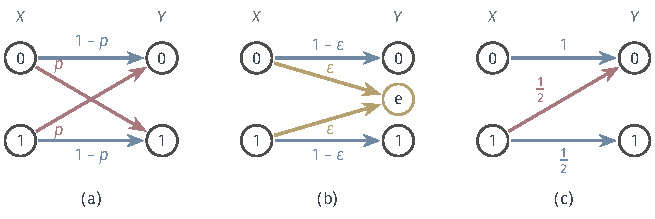
\includegraphics[width=110.9mm]{figures/07-probability/06-channel-coding/tikz/dcc-channel-diagrams/figure.pdf}
 \caption{三个二元输入信道的转移图，箭头上的数是条件概率$W(y\mid x)$。(a) 二元对称信道，红色箭头表示翻转；(b) 二元擦除信道，黄色箭头通向接收端可见的擦除符号$\mathrm{e}$；(c) 本章所用的Z信道，输入$1$以概率$\tfrac12$变成$0$。}
 \label{fig:dcc-channel-diagrams}
\end{BookInlineFigure}

把这些例子的共同结构抽出来：有限的输入字母表、有限的输出字母表，以及每个输入对应的一张输出概率表。

\begin{definition}[离散信道]
\label{def:dcc-channel}
设$\mathcal{X}$、$\mathcal{Y}$是有限集。一个从$\mathcal{X}$到$\mathcal{Y}$的离散信道由一族非负数$W(y\mid x)$给出（$x\in\mathcal{X}$，$y\in\mathcal{Y}$），满足
\begin{equation}
 \sum_{y\in\mathcal{Y}}W(y\mid x)=1,\qquad x\in\mathcal{X} .
 \label{eq:dcc-channel-rows}
\end{equation}
$W(y\mid x)$是输入为$x$时输出为$y$的概率。把它排成$\lvert\mathcal{X}\rvert\times\lvert\mathcal{Y}\rvert$矩阵$\bm{W}$，第$x$行记为$W_x=W(\cdot\mid x)$，称$\bm{W}$为信道的转移矩阵。
\end{definition}

条件~\eqref{eq:dcc-channel-rows}说每一行都是$\mathcal{Y}$上的概率分布。用第~\ref{chap:conditional-distributions}章的语言，$\bm{W}$就是给定$X$时$Y$的条件分布，即一个从$\mathcal{X}$到$\mathcal{Y}$的核；有限字母表上，核就是一张行和为$1$的表。三个例子的转移矩阵依次为
\[
 \begin{pmatrix}1-p&p\\ p&1-p\end{pmatrix},\qquad
 \begin{pmatrix}1-\varepsilon&\varepsilon&0\\ 0&\varepsilon&1-\varepsilon\end{pmatrix},\qquad
 \begin{pmatrix}1&0\\ \tfrac12&\tfrac12\end{pmatrix},
\]
擦除信道的列按输出$0,\mathrm{e},1$排列。

\paragraph{信道固定，输入分布可选}
信道规定的只是“给定输入后输出怎样分布”，至于各个输入多常被使用，由发送端决定。设输入$X$的分布为$q$，即$q(x)=\mathbb{P}(X=x)$，$q$是概率单纯形
\[
 \Delta_{\mathcal{X}}=\Bigl\{q\in\mathbb{R}^{\mathcal{X}}:\ q(x)\geq0,\ \sum_{x}q(x)=1\Bigr\}
\]
中的一点。输入分布与信道合起来确定$(X,Y)$的联合分布与输出分布：
\begin{equation}
 \mathbb{P}(X=x,Y=y)=q(x)W(y\mid x),\qquad
 p_q(y)=\sum_{x\in\mathcal{X}}q(x)W(y\mid x) .
 \label{eq:dcc-output-law}
\end{equation}
写成行向量，$p_q=q\bm{W}$。改变$q$不改变信道，只改变我们如何使用它；后面的容量正是对$q$的最优选择。

式~\eqref{eq:dcc-output-law}说明，输出分布是转移矩阵各行以$q(x)$为权的凸组合。图~\ref{fig:dcc-output-simplex}在输出单纯形中画出这一点。擦除信道$\varepsilon=0.25$的两行是$W_0=(0.75,0.25,0)$与$W_1=(0,0.25,0.75)$，选择$q$只能在连接两行的线段上移动；均匀输入给出中点
\[
 p_q=\tfrac12W_0+\tfrac12W_1=(0.375,\ 0.25,\ 0.375) .
\]
无论怎样选输入，擦除的概率始终是$0.25$：它是信道的性质，输入分布无法改变。

\begin{BookInlineFigure}
 \centering
 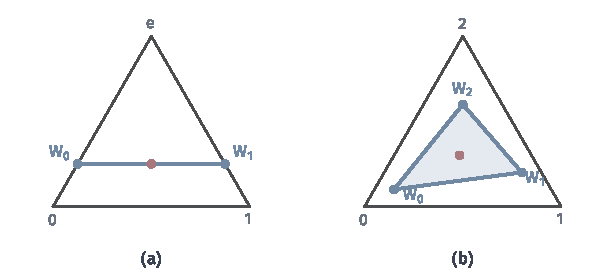
\includegraphics[width=104mm]{figures/07-probability/06-channel-coding/matplotlib/dcc-output-simplex/figure.pdf}
 \caption{输出分布的可达范围。三角形是三个输出上的概率单纯形，顶点是集中于单个输出的分布。(a) 二元擦除信道$\varepsilon=0.25$，蓝点是转移矩阵的两行，蓝线段是$q\bm{W}$的全部可能值；(b) 一个三输入三输出信道，三行为$(0.8,0.1,0.1)$、$(0.1,0.7,0.2)$、$(0.2,0.2,0.6)$，可达的输出分布是浅蓝三角形。红点是均匀输入对应的输出分布。}
 \label{fig:dcc-output-simplex}
\end{BookInlineFigure}

\paragraph{多次使用：无记忆}
传输消息时信道被使用$n$次，输入块$x^n=(x_1,\dots,x_n)$，输出块$y^n=(y_1,\dots,y_n)$。最简单的多次使用规律是：每次使用都经过同一个转移矩阵，各次之间互不影响。

\begin{definition}[离散无记忆信道]
\label{def:dcc-dmc}
以$\bm{W}$为转移矩阵的\term{离散无记忆信道}（discrete memoryless channel）在$n$次使用中，对每个输入块$x^n\in\mathcal{X}^n$，输出块的条件概率为
\begin{equation}
 W^n(y^n\mid x^n)=\prod_{i=1}^{n}W(y_i\mid x_i),\qquad y^n\in\mathcal{Y}^n .
 \label{eq:dcc-memoryless}
\end{equation}
\end{definition}

乘积形式包含两层意思：第$i$个输出只受第$i$个输入影响；给定整个输入块后，各个输出相互独立。以$p=0.1$的二元对称信道为例，发送$111$而收到$101$，需要第一、三位不翻转、第二位翻转，概率是
\[
 W^3(101\mid111)=0.9\times0.1\times0.9=0.081 .
\]

\paragraph{编码器不使用反馈}
式~\eqref{eq:dcc-memoryless}描述的是给定输入块之后输出的规律。还需要说明输入块怎样产生。本章中，发送端在传输之前就由消息确定整个输入块，第$i$次的输入不依赖已经收到的$y_1,\dots,y_{i-1}$。若发送端能看到输出（称为反馈），它可以根据前面的结果调整后面的输入，这时$X_i$与此前的噪声相关，式~\eqref{eq:dcc-memoryless}的乘积结构仍描述每一步的转移，但输入与输出的联合规律不再能直接按块写出，第~\ref{sec:dcc-capacity-formula}节的块互信息上界需要另行论证。图~\ref{fig:dcc-block-system}画出本章的传输结构。

\begin{BookInlineFigure}
 \centering
 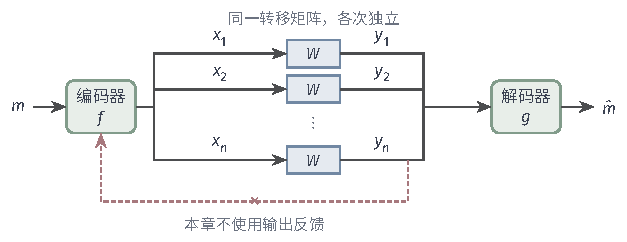
\includegraphics[width=106.2mm]{figures/07-probability/06-channel-coding/tikz/dcc-block-system/figure.pdf}
 \caption{离散无记忆信道上的块传输。编码器$f$把消息$m$一次变成整个输入块，每个符号独立地经过同一转移矩阵$W$，解码器$g$看到整个输出块后给出判决$\hat{m}$。红色虚线表示从输出到编码器的反馈，本章不使用。}
 \label{fig:dcc-block-system}
\end{BookInlineFigure}

无记忆是一个模型假设。若干扰成串出现，例如一次翻转之后紧接着的几个符号也更容易翻转，各次使用就不独立，式~\eqref{eq:dcc-memoryless}不成立。这样的信道需要随机过程的工具描述状态的演化，本章不讨论。
